
\section{Experimentos y Resultados}

Para evaluar el desempeño de la propuesta se evaluó las secuencias con el código \textbf{ERR3014700}, estas fueron descargadas de \href{https://www.ncbi.nlm.nih.gov/sra/ERR3014700}{NCBI}. Estás representan secuencias de \textit{Human betaherpesvirus}. El tamaño de estas secuencis es de 260.3 MB, en formato SRA. Luego fueron descomprimidos con la herramienta SRA de NCBI, como resultado se obtuvo las secuencias en formato FastaQ, en este caso el archivo llego a ocupar 590.8 MB. \\

Luego se levanto el sistema distribuído, se subio el \textit{script} a \textit{spark-submit} y se realizo el análisis. La plataforma retorna como resultado un archivo \textit{json} con detalle del análisis y un gráfico que detalla el análisis de contenido por base. Por ejemplo, para el experimiento mencionado anteriormente, se obtuvo el siguiente \textit{json}. \\

\begin{lstlisting}
{
	"bases": 1843156,
	"total_seqs": 462393,
	"seqs_len": [
		523,
		600,
		599,
		600,
		599,
		600,
		600,
		529,
		600,
		538
	],
	"seqs_len_mean": 564,
	"bases_ocurrence": [
		[
			"C",
			71397200
		],
		[
			"N",
			4054
		],
		[
			"D",
			3004
		],
		[
			"G",
			70502420
		],
		[
			"A",
			59888213
		],
		[
			"F",
			16160
		],
		[
			"T",
			59010438
		],
		[
			"B",
			203
		],
		[
			"E",
			4144
		]
	]
}
\end{lstlisting}


Para el caso del análisis de contenido por base, la plataforma generá el grafico de la Figura 	\ref{fig:analysis2}. Según este análisis, comprobamos que las primeras bases tiene un margen de error (las curvas caen y decaen), luego tambien verificamos que hay posiciones donde la Adenina tiene baja presencia (curva de color rojo),

\begin{figure}[H]
	\centering
	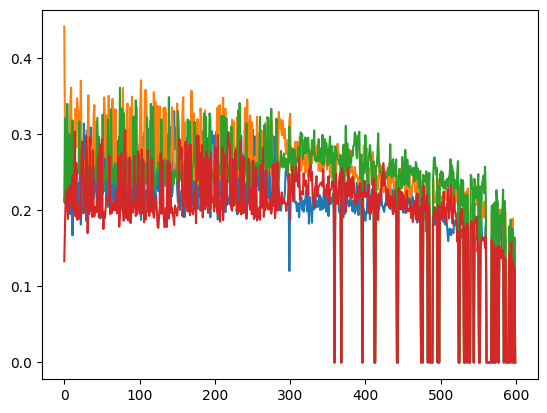
\includegraphics[width=0.6\textwidth]{img/proy/per_base_content}
	\caption{Anĺisis de contenido por base de las secuencias ERR3014700.}
	\label{fig:analysis2}
\end{figure}
